\section{Experimento}
\subsection{Conjunto de datos}

\begin{frame}{DAOs census\footnote{\footcite{tfm-dataset-text}}}
\begin{columns}
\column{.35\linewidth}    
    \begin{itemize}
        \item 30~000 DAOs
        \item 5 millones de votantes
        \item 22 millones de votos emitidos
        \item 180 mil propuestas
    \end{itemize}
\column{.65\linewidth}
\pause
\begin{table}[]
    \centering
    \small
    \begin{tabular}{l|r|r|r|r}
        \textbf{DAO} & 
        \textbf{Props.} & 
        \textbf{Usu.} & 
        \textbf{Vot.} &
        \textperthousand \textbf{Dns.} \\
        \hline
DEAD Foundations      & 5 591 & 3k   & 18k  & 1.83 \\ 
PancakeSwap           & 2 691 & 130k & 533k & 3.05 \\
\textit{Decentraland} & 2 060 & 7k   & 117k & 15.47 \\
AAVE                  & 1 140 & 87k  & 2.3M & 47.28 \\
MetaCartel            &   934 & 200  & 3k   & 35.38 \\
    \end{tabular}
    \caption{Resumen de datos de algunas DAOs}
    \label{tab:my_label}
\end{table}
\end{columns}
\end{frame}

\begin{frame}{Decentraland}
\blfootnote{Fuente: Figuras 4.3 a 4.6 de la memoria}

\begin{itemize}
    \item El 50\% de los 7k usuarios han votado como mucho en 3 propuestas
    \item Las propuestas duran 7 o 14 días
    \item Media de 56 votos por propuesta
    \item Picos de hasta 70 propuestas
    \item Se suelen votar poco después (48 horas) de su fecha de creación
    \item Las propuestas no se crean uniformemente a lo largo del dia de la semana
\end{itemize}
\end{frame}

\subsection{Entrenamiento y validación}

\begin{frame}{División en entrenamiento y prueba}
    \begin{figure}
        \centering
        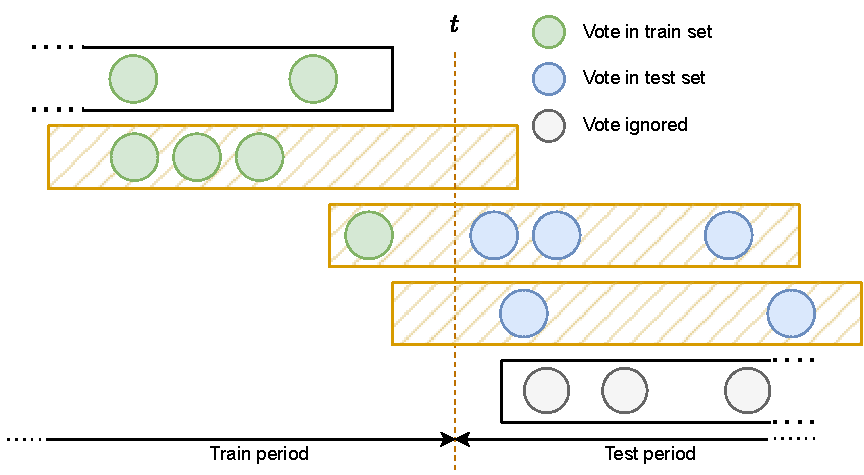
\includegraphics[height=55mm]{images/diagrams/rs-time-folds-evaluacion.drawio.pdf}
        % \caption{Ejemplo de split en \textit{entrenamiento} y \textit{prueba}}
    \end{figure}
\end{frame}


\begin{frame}{Métricas utilizadas}   
\begin{columns}
\column{.4\linewidth}
    \begin{itemize}
        \item precision@k
        \item recall@k
        \item nDCG@k
        \item MAP@k
    \end{itemize}
\column{.6\linewidth}
    \pause
    \centering
    \begin{alertblock}{Cuidado con $k>\left|\text{items rel. en top k}\right|$}
    \begin{equation}
        precision@k=\frac{\left|\text{items rel. en top k}\right|}{k}
    \end{equation}
    \end{alertblock}
\end{columns}
\end{frame}

\begin{frame}{La línea base \textit{OpenPop}}
\begin{columns}
    \column{.5\linewidth}
    \begin{alertblock}{Most Popular no tiene en cuenta:}
    \begin{itemize}
        \item La popularidad en ese momento dado
        \item Si el ítems estaba disponible
        \item Que la prop. puede estar cerrada
    \end{itemize}
    \end{alertblock}
    \column{.5\linewidth}
    \pause
    \begin{exampleblock}{OpenPop}
        Dado un instante $t$, recomendar la propuesta \textbf{abierta} más votada en ese momento siempre que el usuario no haya votado ya en ella.
    \end{exampleblock}
\end{columns}

\blfootnote{\footcite{rendle_difficulty_2019}}
\blfootnote{\footcite{ji_re-visit_2020}}
\end{frame}

\subsection{Implementación y modelos}

\begin{frame}{Modelos}
% \blfootnote{\footcite{aggarwal_recommender_2016}}
\begin{itemize}
    \item<1-> \textbf{Basado en contenido}\onslide<3->{: PLN del texto de las propuestas}
    \item<2-> \textbf{Basado en filtrado colaborativo}\onslide<3->{: Graph Neural Networks (LightGCN)}
    \item<4-> \textbf{Híbrido}: Ensamblaje de los dos anteriores
    % \item<5-> \color{gray}{\textbf{Basado en conocimiento}: No hecho\footnote{\footcite{valiente_integration_2022}}}
\end{itemize}
\end{frame}

\begin{frame}{Modelo basado en contenido}
    TODO: Figura que muestre un ``espacio" 2d o 3d representando los embeddings de las propuestas, y ahí justo en el medio un icono del usuario
\end{frame}

\begin{frame}{Resultados PLN}
    \begin{figure}
        \centering
        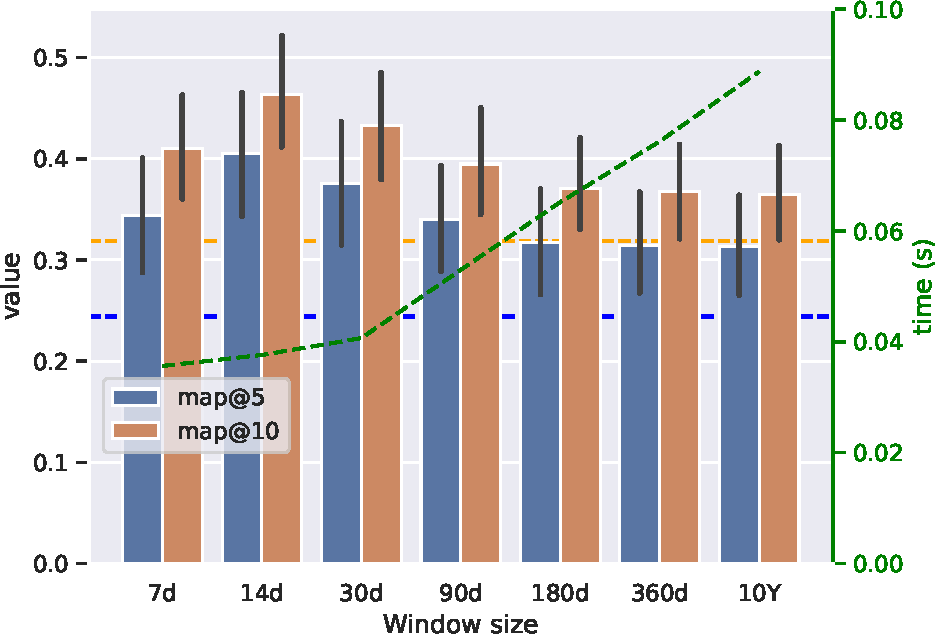
\includegraphics[height=45mm]{./images/graphs/11_cosine_results_window-size_W-THU_normalize=True.pdf}
        \caption{Rendimiento del modelo PLN con respecto al tamaño de la ventana de entrenamiento}
    \end{figure}
\end{frame}

\begin{frame}{Modelo basado en filtrado colaborativo}
    TODO: ¿Pongo la formula de los embeddings y la agregación? Yo creo que sí, la figura del paper también tá chula.
\end{frame}

\begin{frame}{Fine-tuning de LightGCN I}
\begin{table}[]
    \centering
    \begin{tabular}{l|c|c}
\textbf{Hiperparámetro} & \textbf{Valores} & \textbf{Muestreo} \\
\hline
Embedding dim. & $1\leq e\leq 1024, e\in \mathbb{N}$ & Loguniforme \\
Convolution layers & $c\in \{1,2,3,4,5,6\}$ & Uniforme \\
Batch size & $bs\in\{64,128,256,512,1024\}$ & Uniforme \\
Learning rate & $10^{-4}\leq lr\leq 1, lr\in \mathbb{R}$ & Loguniforme \\
L2 regularization & $10^{-7}\leq l2 \leq 10^{-2}, l2 \in \mathbb{R}$ & Loguniforme \\
    \end{tabular}
    \caption{Espacio de búsqueda de hiperparámetros para LightGCN}
\end{table}
\blfootnote{\footcite{bergstra_making_2013}}
\blfootnote{\footcite{liaw_tune_2018}}
\end{frame}

\begin{frame}{Fine-tuning de LightGCN II}
    TODO: Aquí pondré alguna figura que ejemplifique el problema de hyperoptimizar conociendo el futuro o algo así
\end{frame}

\begin{frame}{Fine-tuning de LightGCN III}
    TODO: Aquí pondre como una especie de ``progress bar" que se rellene con distintos colores para indicar la parte que se usa para elegir los hiperparámetros y la que se testea como ``modelo realista''
\end{frame}

\begin{frame}{Resultados GNN}
\begin{columns}
\column{.5\linewidth}
\begin{figure}
    \centering
    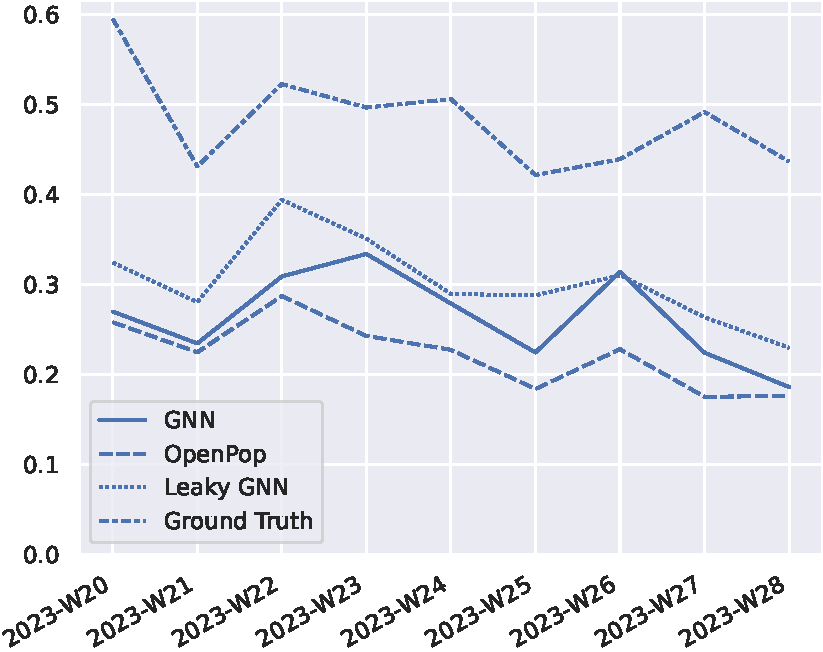
\includegraphics[height=45mm]{./images/graphs/09_gnn_results_precision_5_leaky.pdf}
    \caption{precision@5 del modelo GNN}
\end{figure}
\column{.5\linewidth}
\begin{figure}
    \centering
    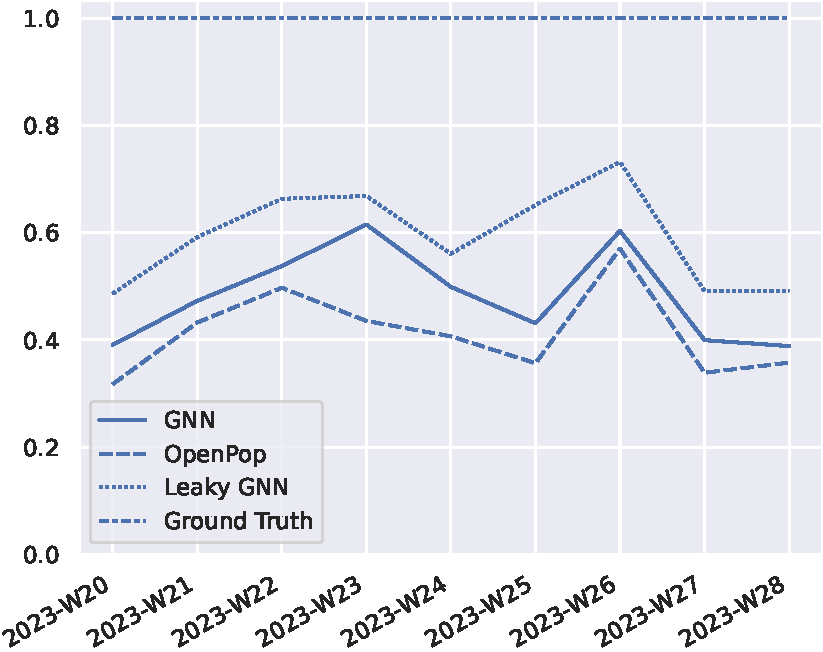
\includegraphics[height=45mm]{./images/graphs/09_gnn_results_ndcg_10_leaky.pdf}
    \caption{ndcg@10 del modelo GNN}
\end{figure}
\end{columns}
\end{frame}

\begin{frame}{Modelo híbrido}
    TODO: Poner la figura 6.9de la memoria (métodos de fusión)
\end{frame}